\documentclass[tikz,border=2pt]{standalone}
\usepackage{amsmath}
\usepackage{pgfplots}
\pgfplotsset{compat=1.18}

\begin{document}
% At a corner the two one-sided derivatives exist but differ: f(x)=|x| has left derivative -1
% and right derivative +1 at 0, so f'(0) does not exist.
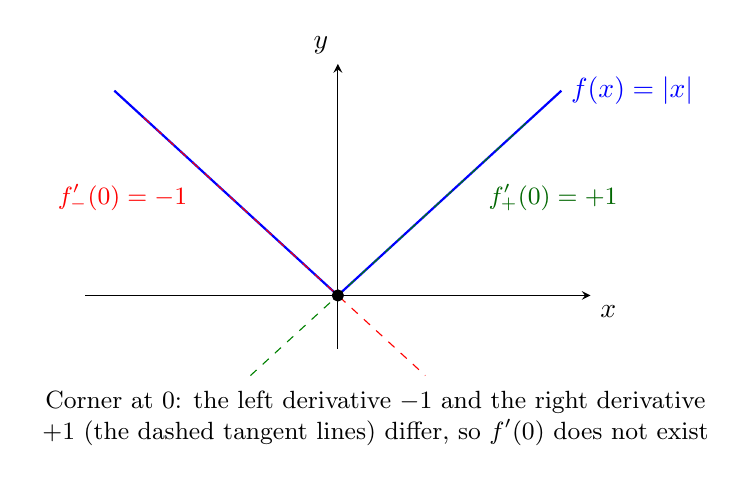
\begin{tikzpicture}
	\begin{axis}[
		axis lines=middle,
		xmin=-2.6, xmax=2.6,
		ymin=-0.6, ymax=2.6,
		xtick=\empty, ytick=\empty,
		xlabel={$x$}, ylabel={$y$},
		xlabel style={below right}, ylabel style={above left},
		samples=2, clip=false,
		width=8cm, height=5.2cm
		]
		\addplot[thick, blue, domain=-2.3:0] {-x};
		\addplot[thick, blue, domain=0:2.3] {x};
		\addplot[red, dashed, domain=-2.0:0.9] {-x};
		\addplot[green!50!black, dashed, domain=-0.9:2.0] {x};
		\addplot[only marks, mark=*, black] coordinates {(0,0)};
		\node[red, anchor=east, font=\small] at (axis cs:-1.45,1.1) {$f'_-(0)=-1$};
		\node[green!40!black, anchor=west, font=\small] at (axis cs:1.45,1.1) {$f'_+(0)=+1$};
		\node[blue, anchor=west] at (axis cs:2.3,2.3) {$f(x)=|x|$};
	\end{axis}
	\node[anchor=north, font=\small, align=flush center, text width=8.6cm] at ([yshift=-2pt]current axis.outer south) {Corner at $0$: the left derivative $-1$ and the right derivative $+1$ (the dashed tangent lines) differ, so $f'(0)$ does not exist};
\end{tikzpicture}
\end{document}
